\begin{center}
    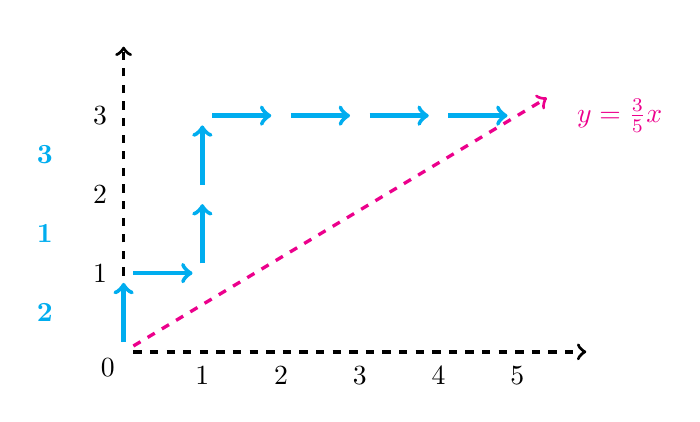
\begin{tikzpicture}[scale=1]
        \node (a) at (0, 0) {};
        \node (b) at (0, 4) {};
        \node (c) at (6, 0) {};
        \node (d) at (5.5, 3.3) {};
        \node (e) at (6.3, 3) [color = magenta]
            {$y = \frac{3}{5}x$}; 
        \draw [dashed, very thick, ->] (a) to (b);
        \draw [dashed, very thick, ->] (a) to (c);
        \draw [dashed, very thick, ->]
            [color = magenta] (a) to (d);

        \node (1)  at (0,0)   {};
        \node (2)  at (0,1)   {};
        \node (3)  at (1,1)   {};
        \node (4)  at (1,2)   {};
        \node (5)  at (1,3)   {};
        \node (6)  at (2,3)   {};
        \node (7)  at (3,3)   {};
        \node (8)  at (4,3)   {};
        \node (9)  at (5,3)   {};
        \draw [->, ultra thick, color = cyan]
            (1)  to (2);
        \draw [->, ultra thick, color = cyan] 
            (2)  to (3);
        \draw [->, ultra thick, color = cyan]
            (3)  to (4);
        \draw [->, ultra thick, color = cyan]
            (4)  to (5);
        \draw [->, ultra thick, color = cyan]
            (5)  to (6);
        \draw [->, ultra thick, color = cyan]
            (6)  to (7);
        \draw [->, ultra thick, color = cyan]
            (7)  to (8);
        \draw [->, ultra thick, color = cyan]
            (8)  to (9);

        \node at (-0.2, -0.2) {$0$};
        \node at (-0.3, 1)    {$1$};
        \node at (1, -0.3)    {$1$};
        \node at (-0.3, 2)    {$2$};
        \node at (2, -0.3)    {$2$};
        \node at (-0.3, 3)    {$3$};
        \node at (3, -0.3)    {$3$};
        \node at (4, -0.3)    {$4$};
        \node at (5, -0.3)    {$5$};

        \node [color = cyan] at (-1, 0.5) {\textbf{2}};
        \node [color = cyan] at (-1, 1.5) {\textbf{1}};
        \node [color = cyan] at (-1, 2.5) {\textbf{3}};
    \end{tikzpicture}
\end{center}